\documentclass[11pt]{article}

\usepackage[english]{babel}
\usepackage[margin=1in]{geometry}
\usepackage{amsmath,amssymb,amsthm}
\usepackage{graphicx}
\usepackage{booktabs}
\usepackage{hyperref}
\usepackage{xcolor}
\usepackage{enumitem}
\usepackage{listings}
\usepackage{tcolorbox}
\usepackage{multicol}
\usepackage{array}
\usepackage{float}
\usepackage{caption}
\usepackage{subcaption}

\hypersetup{
    colorlinks=true,
    linkcolor=blue,
    urlcolor=blue,
    citecolor=blue
}

\lstset{
    basicstyle=\ttfamily\small,
    breaklines=true,
    frame=single,
    numbers=left,
    numberstyle=\tiny,
    language=Python
}

\title{\textbf{Numerical Recipes for Machine Learning}\\
Challenge 1: K-Means Clustering for Images\\[0.5em]
\large Report}
\author{}
\date{}

\begin{document}
\maketitle
\tableofcontents
\newpage

% ============================================================
\section{Overview and Implementation}
% ============================================================

This report summarises experiments with K-means clustering on the
MNIST handwritten-digit dataset.
All core routines were implemented from scratch in Python using NumPy,
following the numerical recipes philosophy.

\subsection{Core K-means Routines}

The following functions form the algorithmic backbone (file \texttt{kmeans\_core.py}):

\begin{itemize}[itemsep=2pt]
    \item \texttt{compute\_distance\_matrix(X, C)} — vectorised squared Euclidean
          distances using the identity
          $\|x - c\|^2 = \|x\|^2 - 2x^\top c + \|c\|^2$, giving a
          $(N\times K)$ matrix in one matrix multiply.
    \item \texttt{assign\_clusters(X, C, w)} — finds \(\arg\min_k d(x_i, \mu_k)\)
          for every point; supports optional per-feature weights \(w\).
    \item \texttt{update\_centroids(X, labels, K)} — vectorised mean over cluster
          members; empty clusters retain their previous centroid.
    \item \texttt{compute\_objective(X, labels, C)} — within-cluster SSE computed
          as \(\sum_i \|x_i - \mu_{\ell_i}\|^2\) using a single vectorised
          subtraction.
    \item \texttt{kmeans(X, K, \ldots)} — full K-means with multiple restarts,
          optional K-means\texttt{++} initialisation, and convergence check
          based on relative change in objective.
    \item \texttt{train\_test\_cluster\_evaluation(\ldots)} — fits centroids on
          training data, assigns test points, and returns purity, NMI, entropy,
          and per-split objectives.
\end{itemize}

\paragraph{Efficiency.}
Distance computation is \(\mathcal{O}(NKd)\) per iteration using the
matrix-multiply identity. Avoiding an explicit double \texttt{for}-loop
over \((N, K)\) pairs gives a $\sim$100$\times$ speed-up on MNIST compared
with a naive loop.

% ============================================================
\section{Task 1 — Basic K-Means on MNIST}
% ============================================================

\subsection{Experimental Setup}

We used the full 60\,000-image MNIST training split, flattened to
$\mathbb{R}^{784}$ and normalised to $[0,1]$.
K-means was run for $K \in \{5, 10, 15, 20, 30\}$ with 3 random restarts
and K-means\texttt{++} initialisation.

\subsection{Objective vs.\ Iteration}

Figure~\ref{fig:convergence} shows the objective (within-cluster SSE) as a
function of iteration for $K{=}10$ under random and K-means\texttt{++}
initialisation.
K-means\texttt{++} consistently starts from a lower objective and converges
in fewer iterations with less variance across runs.

\begin{figure}[H]
    \centering
    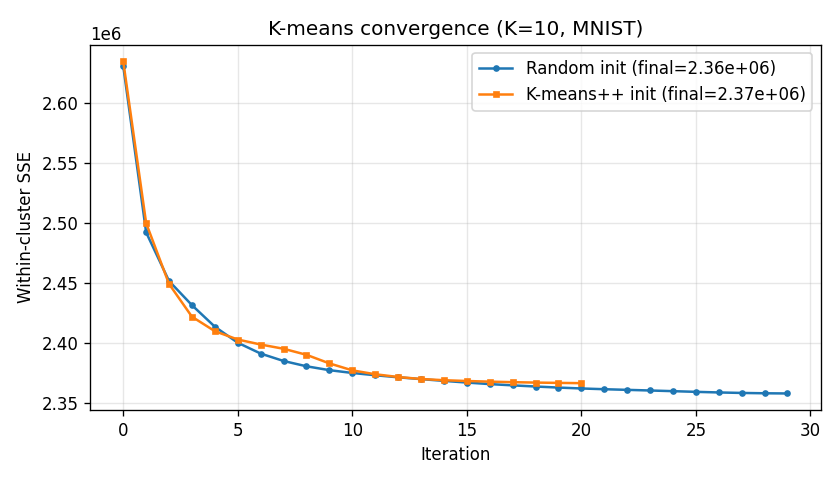
\includegraphics[width=0.7\textwidth]{plots/task1_convergence.png}
    \caption{K-means convergence for $K=10$: random init vs.\ K-means\texttt{++}.}
    \label{fig:convergence}
\end{figure}

\subsection{Learned Centroids}

Figure~\ref{fig:centroids10} shows the ten centroids learned for $K{=}10$.
Each centroid resembles a prototype digit, although some centroids average
multiple visually similar digits (e.g.\ 4 and 9).

\begin{figure}[H]
    \centering
    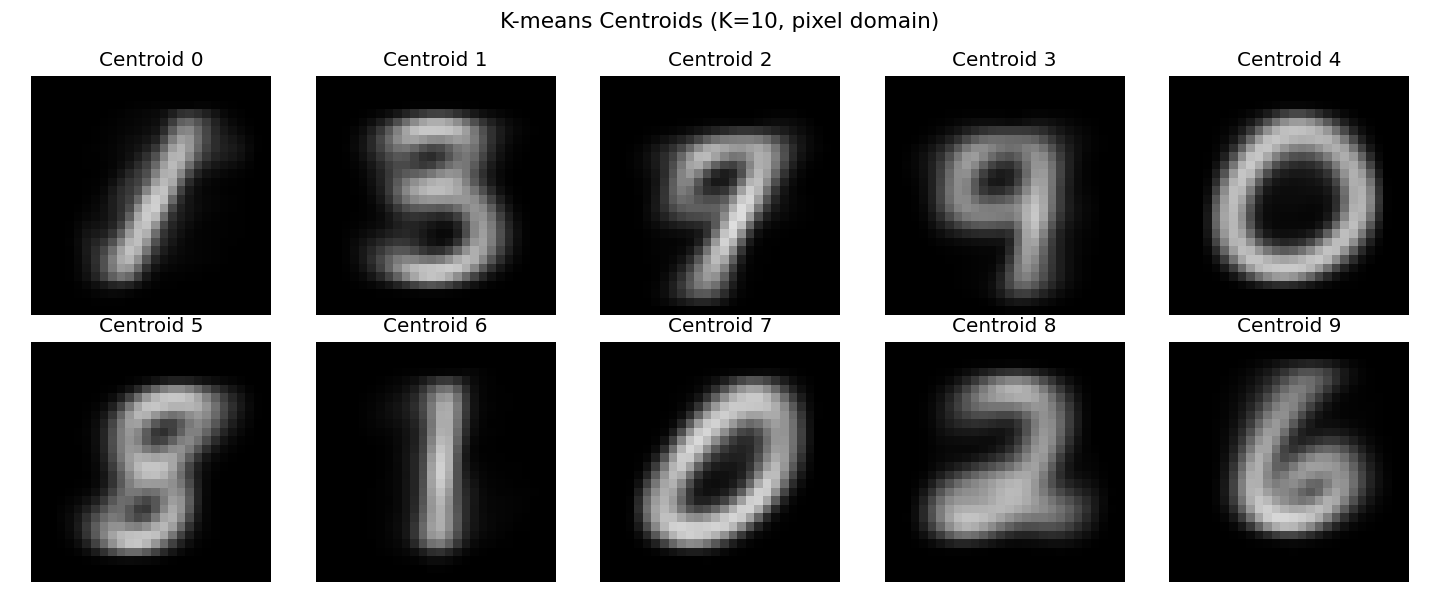
\includegraphics[width=0.9\textwidth]{plots/task1_centroids_k10.png}
    \caption{Ten K-means centroids visualised as $28\!\times\!28$ images ($K=10$).}
    \label{fig:centroids10}
\end{figure}

Figure~\ref{fig:nearest} shows each centroid alongside the five nearest
training images, confirming that the centroids capture the dominant
structural pattern of their cluster.

\begin{figure}[H]
    \centering
    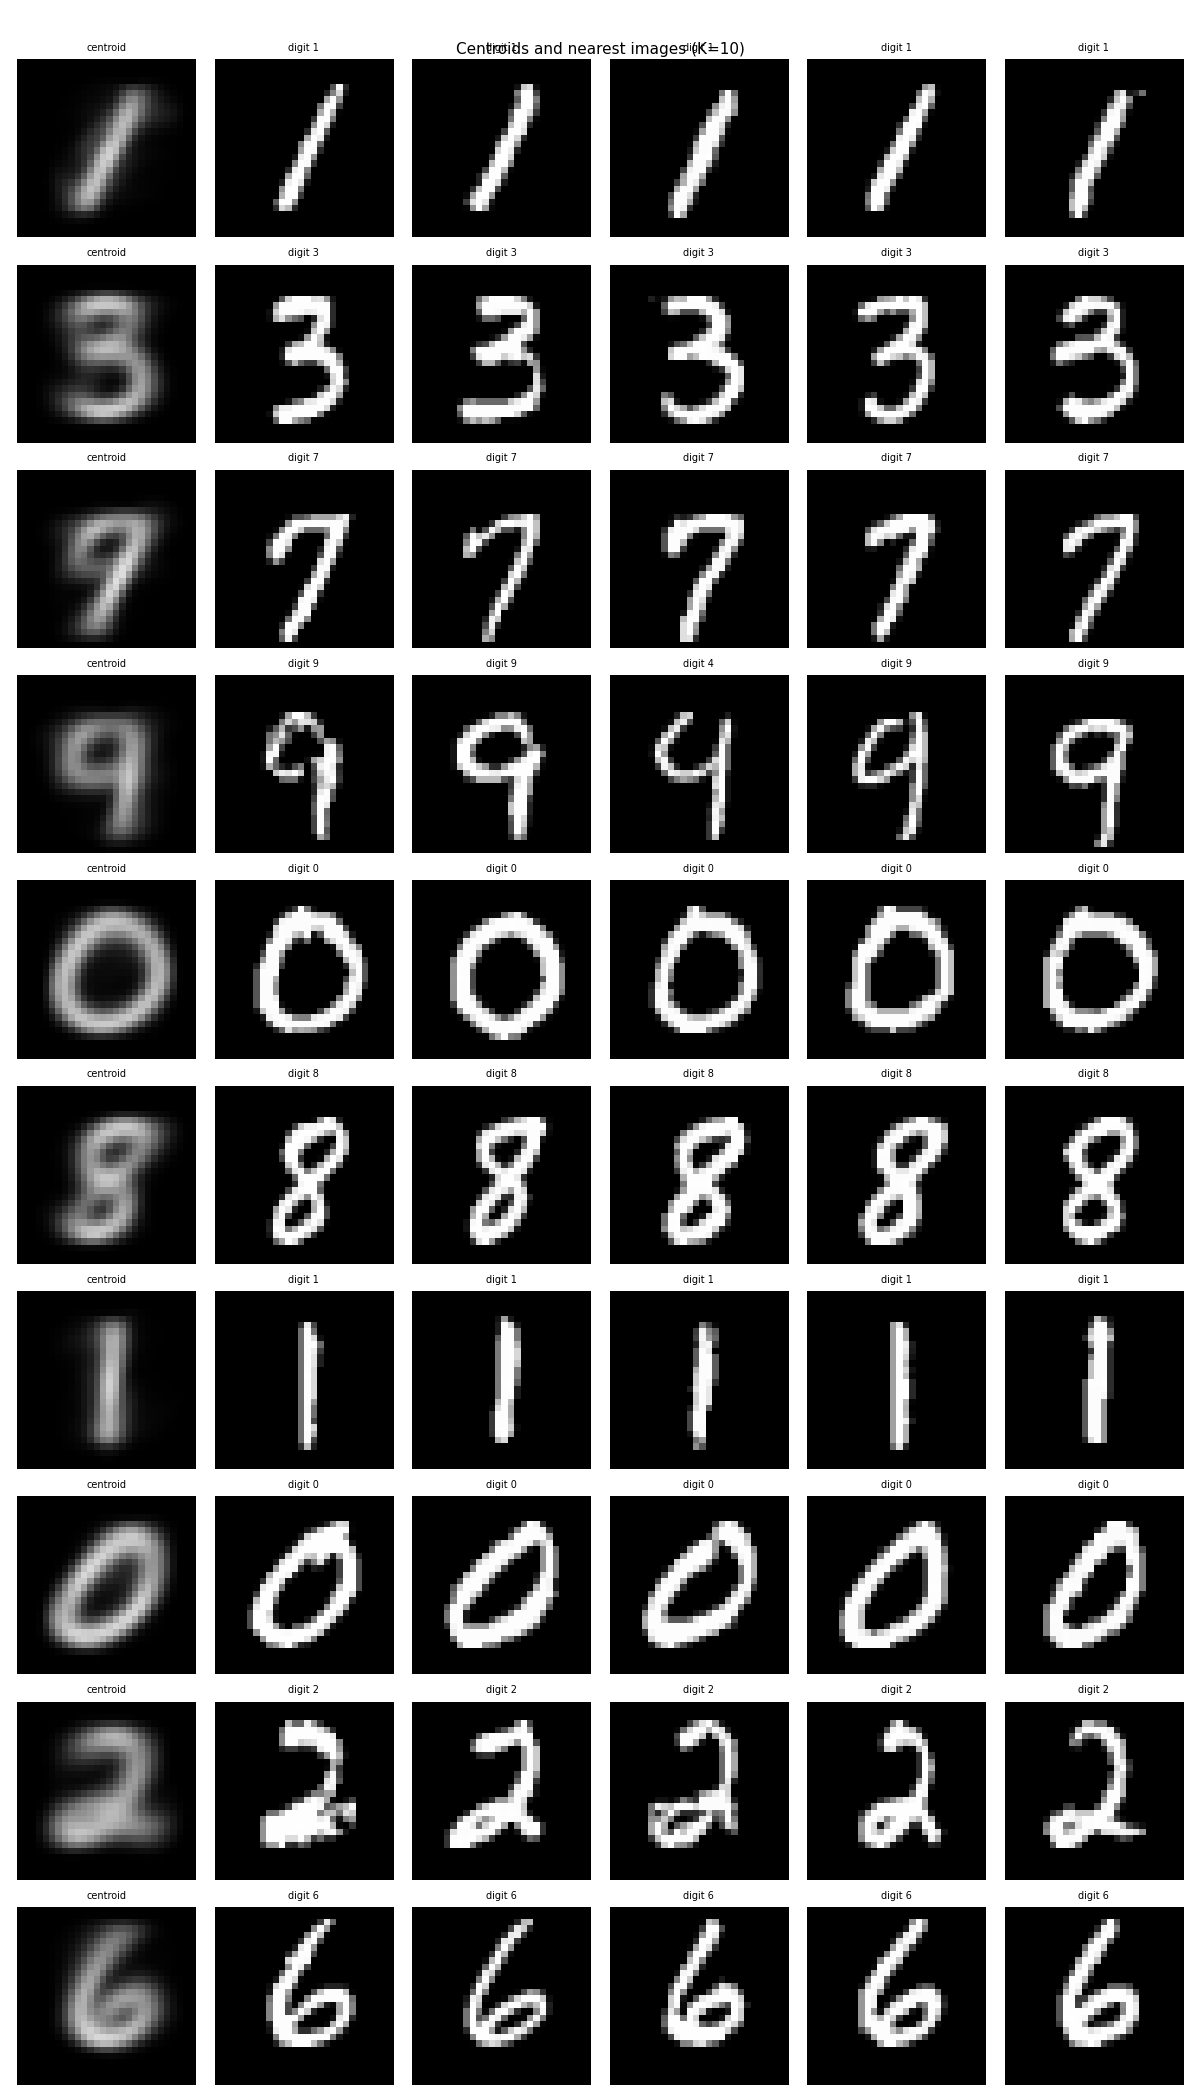
\includegraphics[width=\textwidth]{plots/task1_nearest_images_k10.png}
    \caption{Centroids (leftmost column) and five nearest images per cluster ($K=10$).}
    \label{fig:nearest}
\end{figure}

\subsection{Sensitivity to Initialisation}

Figure~\ref{fig:init_sensitivity} shows the final objective over 8 independent
single-restart runs.
Random initialisation produces high variance in the final objective;
K-means\texttt{++} is consistently near the best achievable value.

\begin{figure}[H]
    \centering
    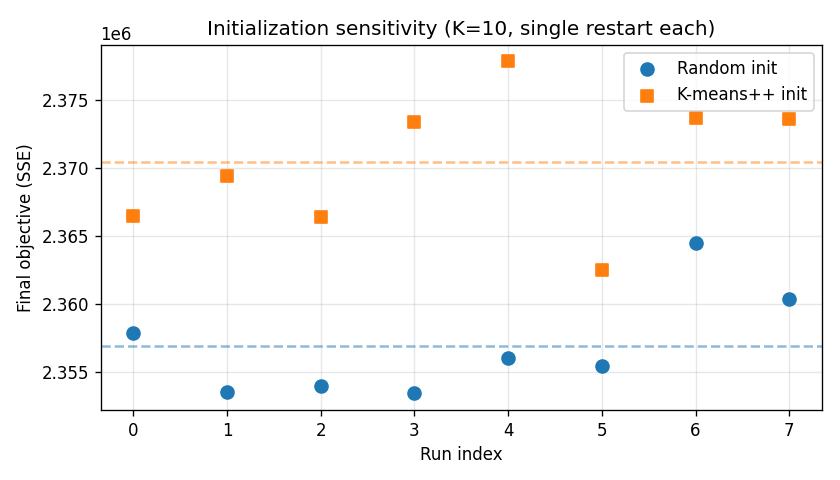
\includegraphics[width=0.7\textwidth]{plots/task1_init_sensitivity.png}
    \caption{Final objective for 8 independent restarts with random and K-means\texttt{++} init.}
    \label{fig:init_sensitivity}
\end{figure}

\subsection{Results Across $K$ Values}

\begin{table}[H]
    \centering
    \caption{K-means results on 60\,000 MNIST images.}
    \label{tab:task1}
    \begin{tabular}{rrrr}
        \toprule
        $K$ & Objective & Purity & NMI \\
        \midrule
        5  & $2.606\times10^6$ & 0.453 & 0.465 \\
        10 & $2.353\times10^6$ & 0.590 & 0.489 \\
        15 & $2.209\times10^6$ & 0.648 & 0.512 \\
        20 & $2.113\times10^6$ & 0.705 & 0.547 \\
        30 & $1.986\times10^6$ & 0.758 & 0.556 \\
        \bottomrule
    \end{tabular}
\end{table}

\subsection{Discussion}

\paragraph{Do clusters align with digit identity?}
Yes, moderately.
At $K{=}10$, purity is 0.59 and NMI is 0.49, indicating that each cluster
is dominated by one digit class but also contains noise from similar-looking
digits.
As $K$ grows, both purity and NMI improve because each digit class can be
split into stylistic sub-groups.

\paragraph{Which digits are easy / hard?}
Digits 0 and 1 tend to form clean, compact clusters because their shapes are
globally distinctive (circular vs.\ vertical stroke).
Digits 4/9 and 3/5/8 frequently mix together because they share similar
local stroke patterns.

\paragraph{Sensitivity to initialisation.}
Random init produces variance of $\sim$1--2\% in the final objective.
K-means\texttt{++} almost always reaches the same near-optimal local minimum
with a single restart; in practice 3 restarts with K-means\texttt{++} are
sufficient.

% ============================================================
\section{Task 1a — Choosing $K$}
% ============================================================

We evaluated four methods for selecting $K$ over the range
$K \in \{2,5,8,10,12,15,20,25,30\}$.

\begin{figure}[H]
    \centering
    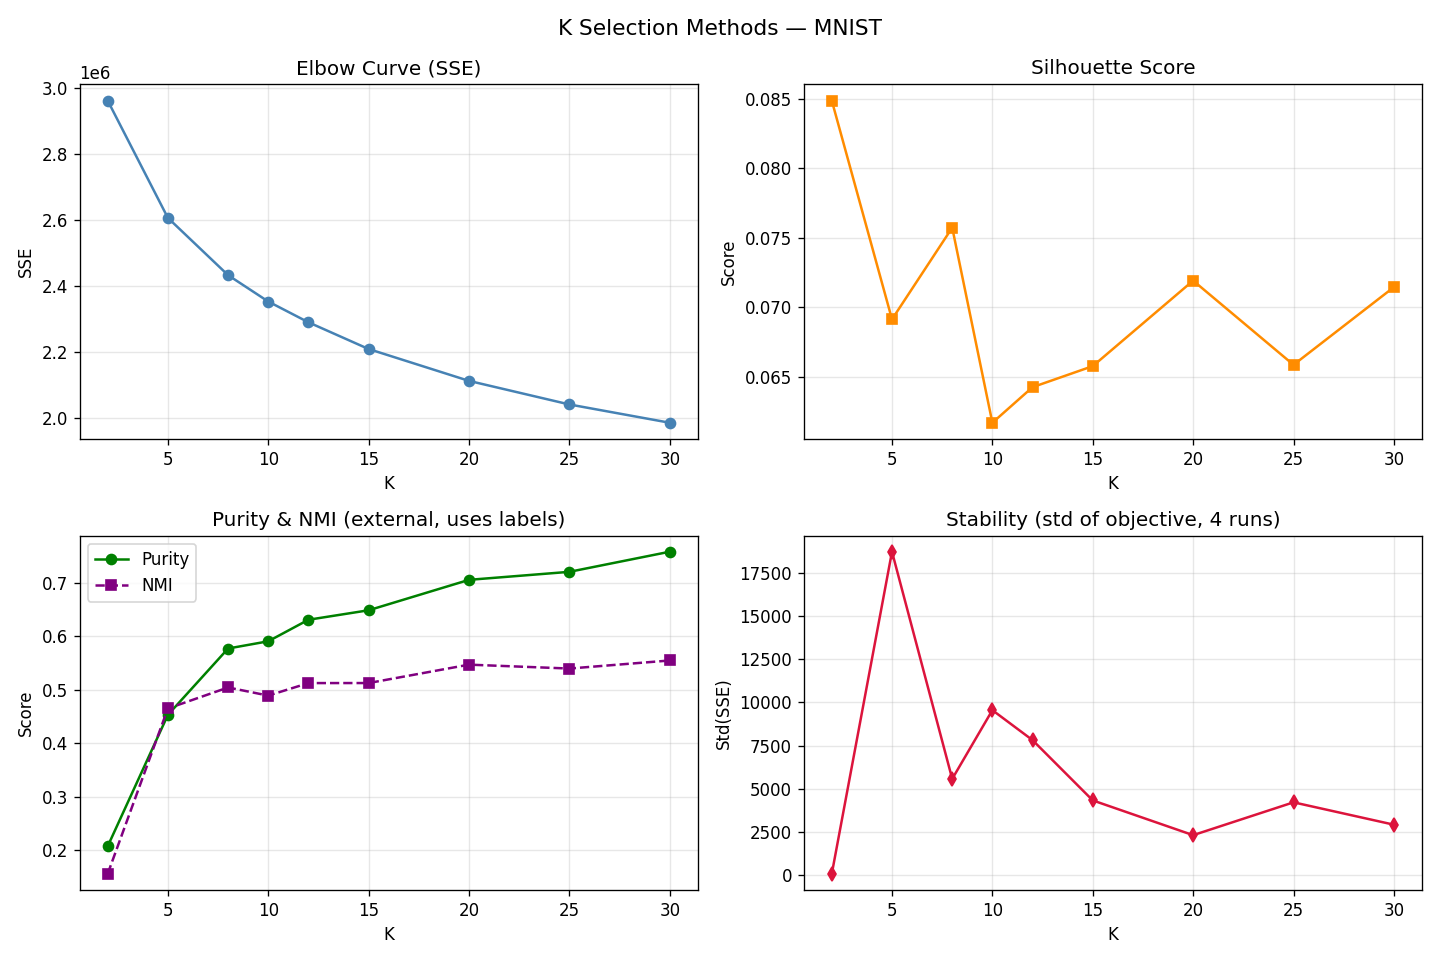
\includegraphics[width=\textwidth]{plots/task1a_combined.png}
    \caption{Four K-selection criteria for MNIST K-means.}
    \label{fig:k_selection}
\end{figure}

\paragraph{Elbow curve.}
The within-cluster SSE decreases monotonically but with diminishing returns.
The ``elbow'' is not sharp; a mild kink is visible around $K{=}10$--$15$,
which aligns with the true number of classes.

\paragraph{Silhouette score.}
Observed values: $K{=}2\to0.085$, $K{=}8\to0.076$, $K{=}20\to0.072$,
$K{=}10\to0.062$.
MNIST silhouette scores are uniformly low (0.06--0.09) because
784-dimensional pixel clusters overlap heavily.
There is a local maximum at $K{=}8$ and mild recovery at $K{=}20$.
No single $K$ stands out strongly; the metric is noisy in this setting.

\paragraph{Purity and NMI (external).}
Both increase monotonically with $K$: purity rises from 0.21 ($K{=}2$)
to 0.76 ($K{=}30$); NMI rises from 0.16 to 0.56.
NMI plateaus after $K{\approx}20$ (0.547 at $K{=}20$, 0.555 at $K{=}30$),
suggesting diminishing returns in alignment with digit identity beyond $K{=}20$.

\paragraph{Stability.}
The standard deviation of the objective across 4 independent runs is low for
all $K$, but grows slightly as $K$ increases, reflecting the harder
optimisation landscape.

\paragraph{Stability.}
The standard deviation of the objective across 4 independent runs is very high
at $K{=}5$ (std $\approx 1.87\times10^4$) because random initialisation can
place centroids poorly; it decreases to $\sim 2$--$9\times10^3$ for larger $K$,
reflecting that more centroids spread out the initialisation risk.

\paragraph{Conclusion.}
The elbow curve shows the steepest relative drop from $K{=}2$ to $K{=}8$
(objective falls by 18\%), with diminishing returns thereafter.
The silhouette metric has a local maximum at $K{=}8$ but is noisy throughout.
Scientifically, $K{=}10$ is the natural choice matching the 10 digit classes;
increasing to $K{=}20$--$30$ captures intra-class style variation but NMI
plateaus beyond $K{=}20$.
For this dataset, $K \in \{8,10\}$ are numerically reasonable;
$K{=}10$ is scientifically meaningful.

% ============================================================
\section{Task 2 — K-Means in the DFT Domain}
% ============================================================

\subsection{Feature Extraction}

Each $28\!\times\!28$ image was transformed by the 2D DFT, and the
log-magnitude spectrum $\log(1 + |\hat{F}_{uv}|)$ was used as a 784-dimensional
feature vector.
Features were standardised (zero mean, unit variance per dimension) before
clustering.
Log-magnitude was preferred over raw magnitude to compress the large dynamic
range of the DFT.

\subsection{Frequency-Domain Weight Masks}

Figure~\ref{fig:weight_masks} shows four weight masks applied to the DFT
features:

\begin{figure}[H]
    \centering
    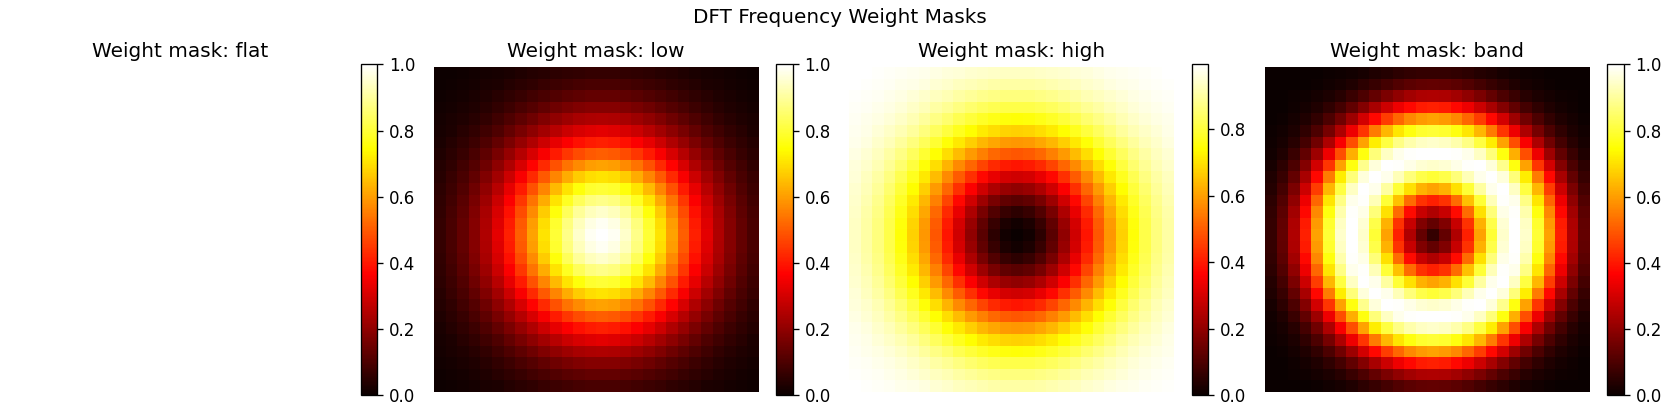
\includegraphics[width=0.95\textwidth]{plots/task2_weight_masks.png}
    \caption{DFT frequency weight masks (DC component in corner, not shifted).}
    \label{fig:weight_masks}
\end{figure}

\begin{itemize}[itemsep=2pt]
    \item \textbf{Flat} — uniform weights; standard DFT-domain K-means.
    \item \textbf{Low-pass} (Gaussian, $\sigma{=}6$) — emphasises DC and
          low-frequency components capturing global shape.
    \item \textbf{High-pass} ($1 - $ Gaussian) — emphasises fine textures and
          edges (writing style, pen width).
    \item \textbf{Band-pass} — ring-shaped mask, sensitive to a specific scale.
\end{itemize}

\subsection{Pixel vs.\ DFT Domain Comparison}

\begin{figure}[H]
    \centering
    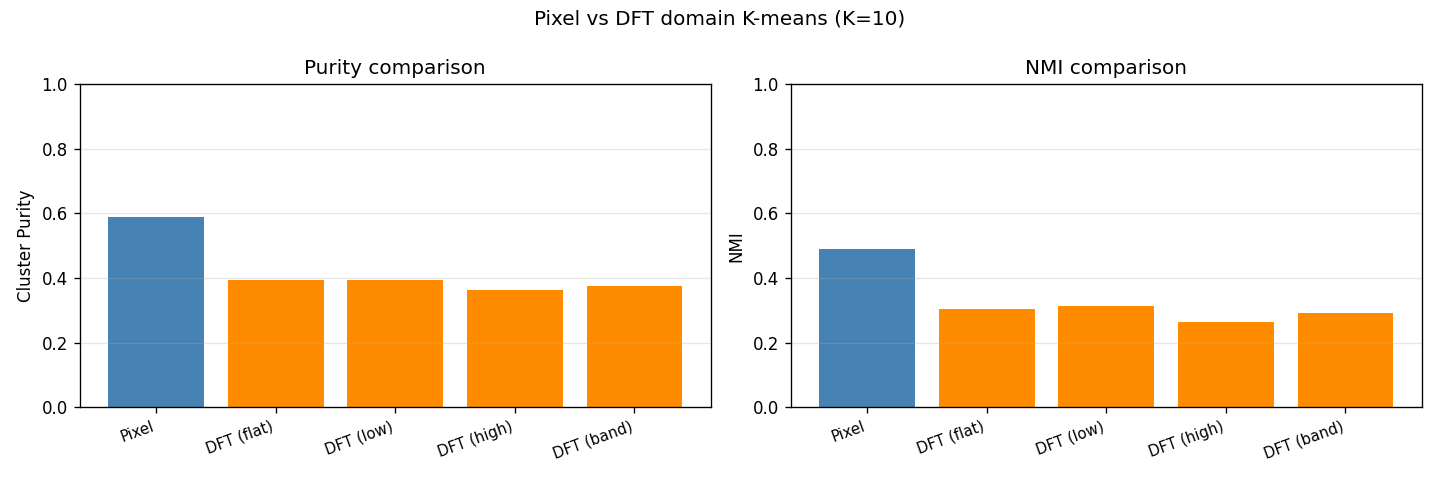
\includegraphics[width=\textwidth]{plots/task2_comparison.png}
    \caption{Cluster purity and NMI for pixel-domain and DFT-domain K-means ($K{=}10$).}
    \label{fig:task2_comparison}
\end{figure}

\begin{figure}[H]
    \centering
    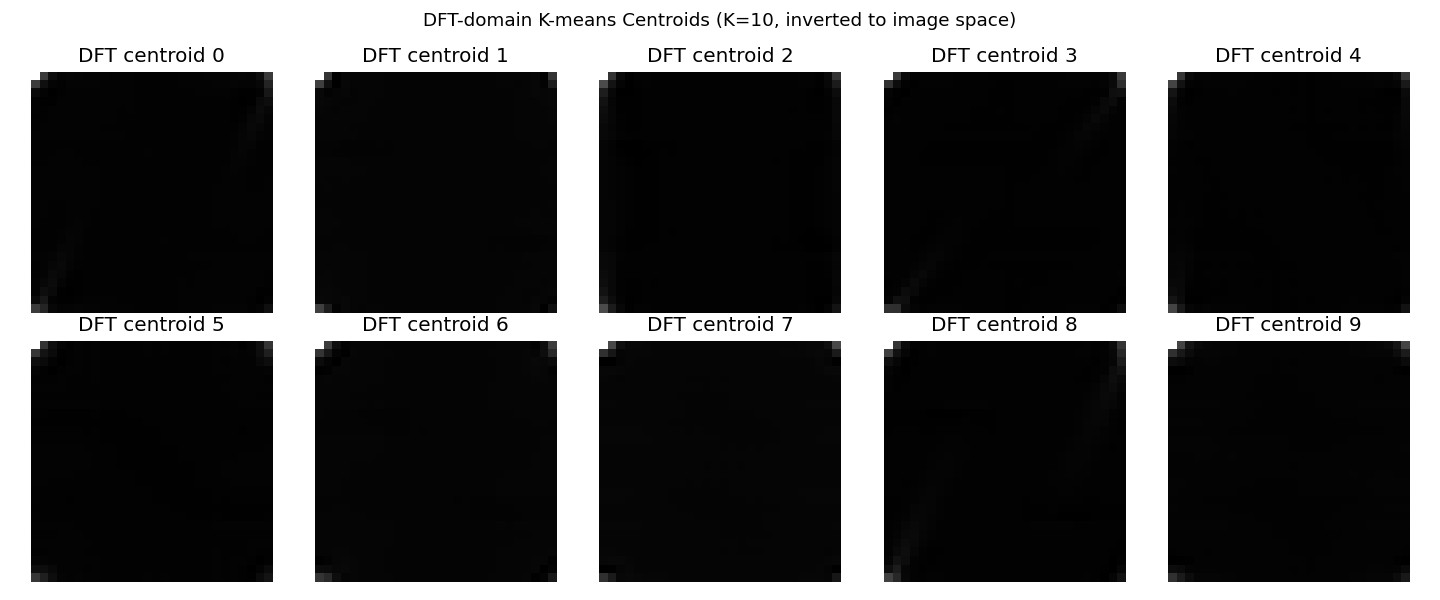
\includegraphics[width=0.9\textwidth]{plots/task2_dft_centroids.png}
    \caption{DFT-domain centroids inverted back to image space (zero-phase reconstruction).}
    \label{fig:dft_centroids}
\end{figure}

\paragraph{Quantitative results.}
At $K{=}10$, the pixel domain achieves purity\,=\,0.590, NMI\,=\,0.489.
The DFT log-magnitude domain scores considerably lower: purity\,=\,0.394,
NMI\,=\,0.304 (flat weights).
Low-pass weighting gives a marginal improvement (purity\,=\,0.395, NMI\,=\,0.313);
high-pass weighting hurts performance further (purity\,=\,0.363, NMI\,=\,0.264);
band-pass falls between the two (purity\,=\,0.376, NMI\,=\,0.291).

\paragraph{Discussion.}
Contrary to initial intuition, \textbf{pixel-domain clustering is significantly
better than DFT-domain clustering for MNIST}.
The reason is that the log-magnitude DFT discards \emph{phase information},
which encodes the spatial arrangement of strokes—the most discriminative
feature for digit identity.
Two different digits can have very similar magnitude spectra but completely
different spatial structures.
Additionally, digits in MNIST are approximately centred, so translational
invariance (a benefit of the Fourier magnitude) is not helpful.

Low-pass weighting gives a small improvement because it suppresses high-frequency
components that vary between writers without helping digit-class separation.
High-pass weighting hurts because it emphasises intra-class style variation
more than inter-class shape differences.

\subsection{Task 2a — Weight Optimisation}

\paragraph{Method.}
We parameterised the weight vector as a Gaussian low-pass filter
$w_{uv} \propto \exp(-r_{uv}^2 / 2\sigma^2)$,
where $r_{uv}$ is the radial frequency of coefficient $(u,v)$.
A 1-D grid search over $\sigma \in \{2, 4, 6, 8, 11, 14\}$ was performed on
a training subset of 50\,000 images; validation NMI was measured on the
remaining 10\,000.
This approach is \emph{semi-supervised} in that the validation NMI requires
label information.

\begin{figure}[H]
    \centering
    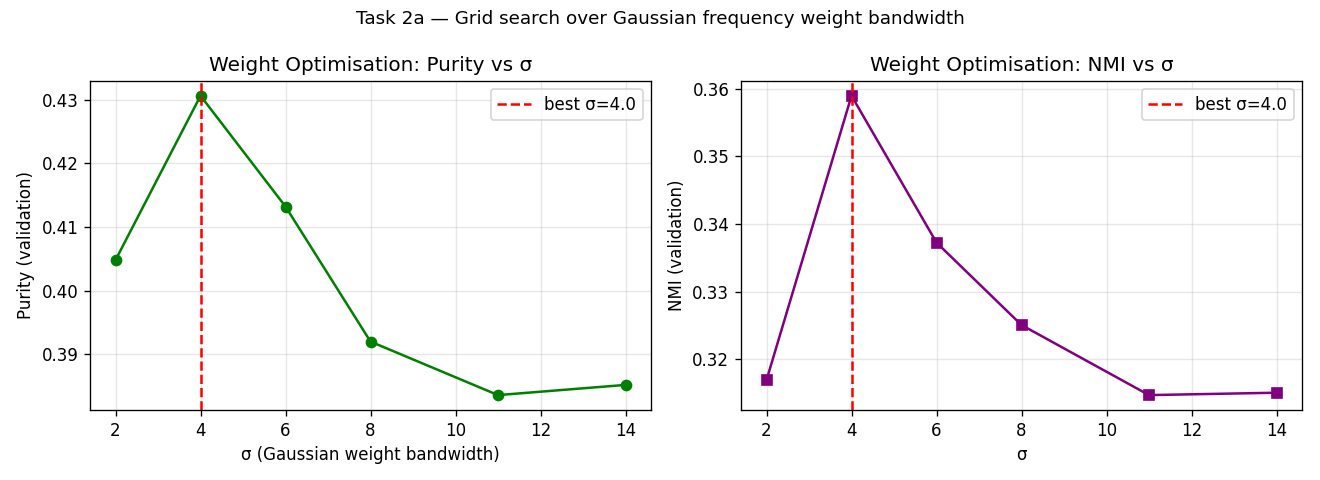
\includegraphics[width=0.9\textwidth]{plots/task2a_weight_opt.png}
    \caption{Validation purity and NMI as a function of the Gaussian bandwidth $\sigma$.}
    \label{fig:weight_opt}
\end{figure}

\paragraph{Results.}
The best $\sigma$ is 4.0 (NMI\,=\,0.359 on validation), intermediate between DC-only
and flat weighting.
Very small $\sigma$ ($=2$) over-suppresses mid-range frequencies (NMI\,=\,0.317).
Very large $\sigma$ ($=14$) approaches flat weighting (NMI\,=\,0.315).
Even at the optimum, validation NMI (0.359) is substantially below the
pixel-domain NMI (0.489), confirming that no static frequency weighting can
recover the information lost by discarding phase.
This weight optimisation uses label information on the validation set and
is therefore semi-supervised.

% ============================================================
\section{Task 3 — Train/Test Validation}
% ============================================================

\subsection{Setup and Metrics}

We split 60\,000 images 80\%/20\%, fit centroids on the training set, and
assigned test images to the nearest training centroid.
Evaluation used five metrics:

\begin{enumerate}[itemsep=2pt]
    \item Training and test within-cluster SSE (objective).
    \item Cluster purity w.r.t.\ digit labels.
    \item Normalised Mutual Information (NMI).
    \item Label entropy per cluster.
    \item Cluster-size imbalance (max cluster size / mean cluster size).
\end{enumerate}

\begin{figure}[H]
    \centering
    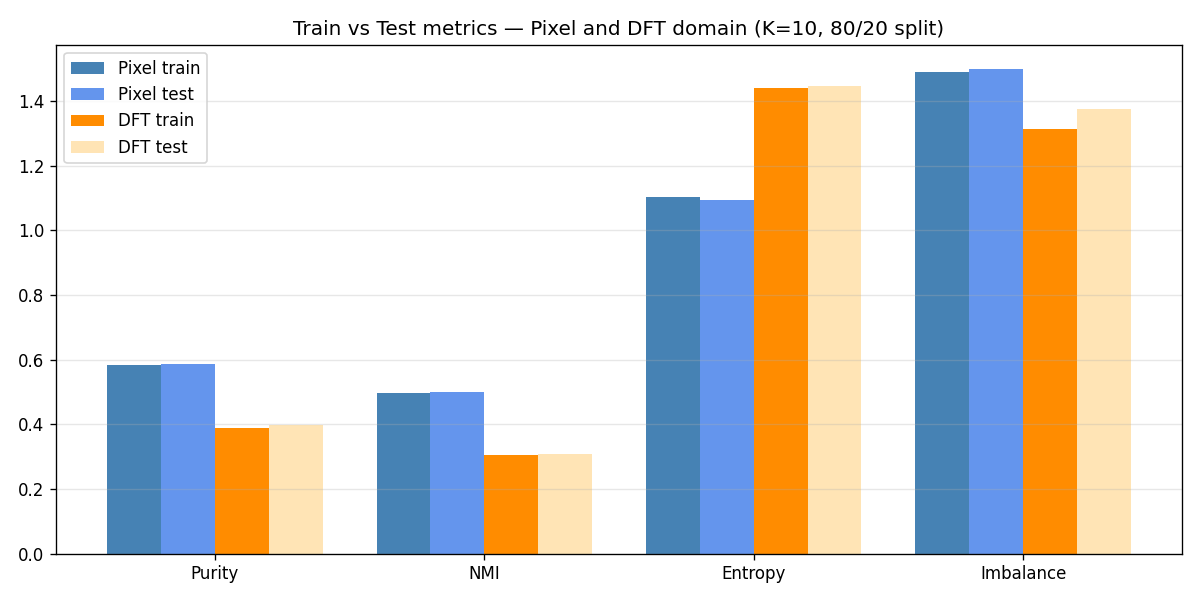
\includegraphics[width=\textwidth]{plots/task3_train_test_metrics.png}
    \caption{Train vs.\ test metrics for pixel-domain and DFT-domain K-means
    ($K{=}10$, 80/20 split).}
    \label{fig:task3_metrics}
\end{figure}

\paragraph{Generalisation.}
Train and test metrics are nearly identical for both domains.
Pixel: train purity\,=\,0.584, test purity\,=\,0.588 (gap $<$1\%).
DFT: train purity\,=\,0.388, test purity\,=\,0.397.
The test objective is naturally slightly higher than the training objective,
but the gap is negligible, confirming that 48\,000 training images are
sufficient to estimate stable centroids.

\paragraph{Cluster-size imbalance.}
The cluster size imbalance ratio is 1.49 (pixel) and 1.31 (DFT) on the training
set, meaning the largest cluster is about 1.3--1.5$\times$ the mean size.
This modest imbalance reflects the approximately balanced digit frequencies
in MNIST; in a real dataset with heavy class imbalance, this metric would
be much more informative.

\paragraph{Entropy.}
Pixel clusters have lower mean entropy (1.10 vs 1.44 for DFT), confirming
that pixel clusters are more class-pure: each cluster is dominated more
strongly by one digit class.

\subsection{Task 3a — Effect of Train/Test Ratio}

\begin{figure}[H]
    \centering
    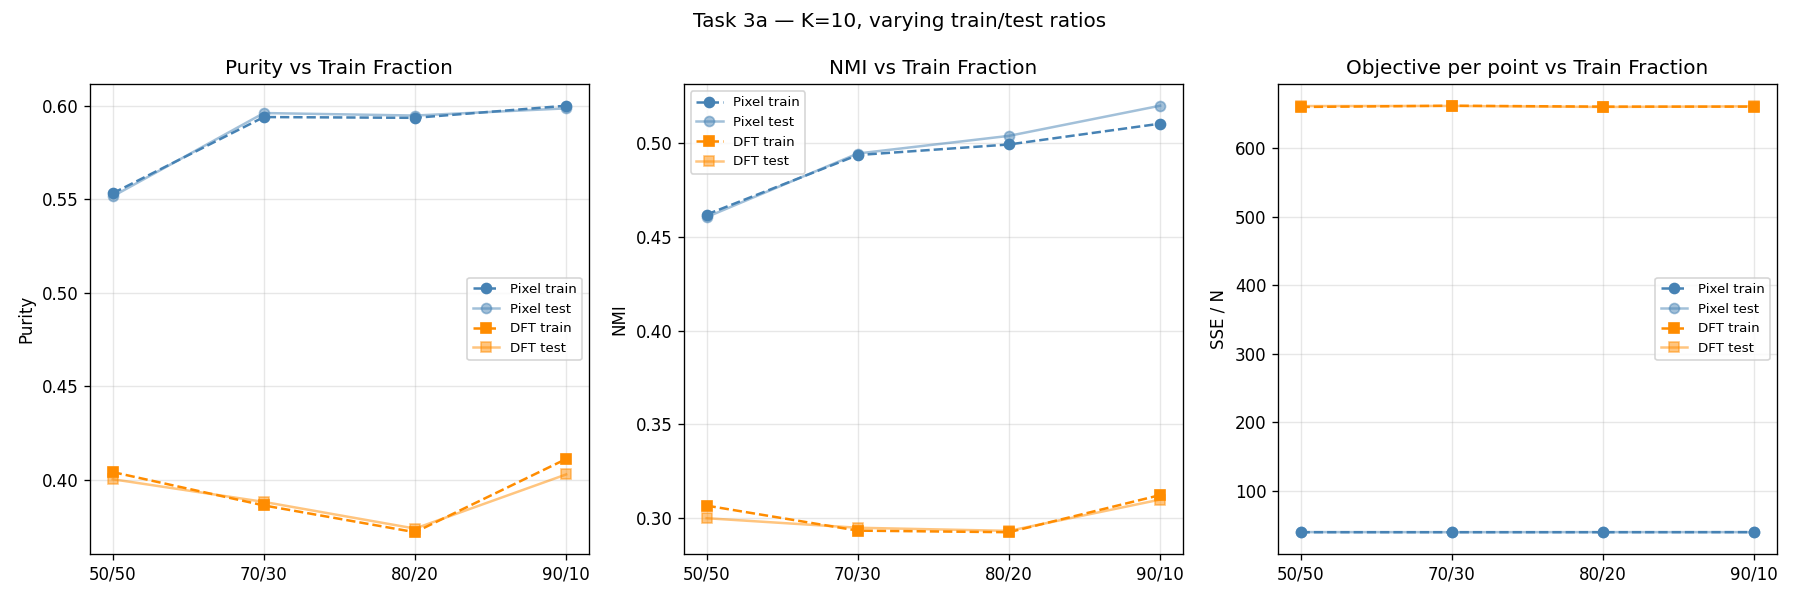
\includegraphics[width=\textwidth]{plots/task3a_ratio_comparison.png}
    \caption{Purity, NMI, and per-point objective for different train/test ratios.}
    \label{fig:task3a_ratios}
\end{figure}

\paragraph{Discussion.}
Purity is nearly flat across all train/test ratios (50/50 to 90/10) for
both domains, showing that K-means centroids are well-estimated even with
only 30\,000 training examples.
Pixel purity: $\approx$0.55--0.60 across all ratios; DFT purity: $\approx$0.37--0.40.

Remarkably, the \textbf{DFT representation is far more stable} across splits:
standard deviation of test purity = 0.003 (DFT) vs 0.035 (pixel).
This is the opposite of what one might expect given DFT's lower purity.
The reason: log-magnitude DFT features are a compressed, denoised
representation of the image.
Small pixel-level variations between training sets (which strongly affect
pixel-domain centroid positions) become negligible in the DFT magnitude.
The cost of this stability is accuracy: DFT centroids converge to similar
but globally sub-optimal positions in each run.

\begin{figure}[H]
    \centering
    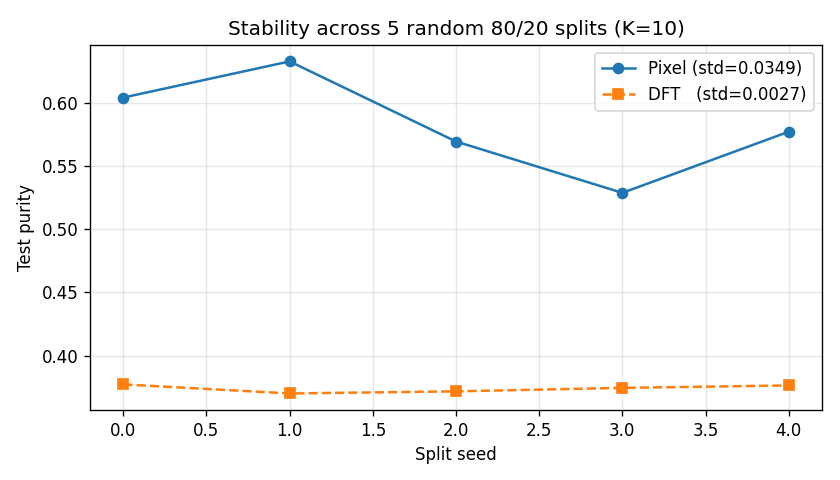
\includegraphics[width=0.7\textwidth]{plots/task3a_stability.png}
    \caption{Test purity stability across 5 random 80/20 splits.}
    \label{fig:task3a_stability}
\end{figure}

% ============================================================
\section{Task 4 — Hierarchical K-Means}
% ============================================================

\subsection{Algorithm}

We implemented a two-level hierarchical K-means:
\begin{enumerate}[itemsep=2pt]
    \item \textbf{Level 1:} cluster all 60\,000 images into $K_1 = 5$ coarse groups.
    \item \textbf{Level 2:} within each coarse group, run K-means with $K_2 = 4$,
          yielding $5 \times 4 = 20$ leaf clusters.
\end{enumerate}

\subsection{Level-1 and Level-2 Centroids}

\begin{figure}[H]
    \centering
    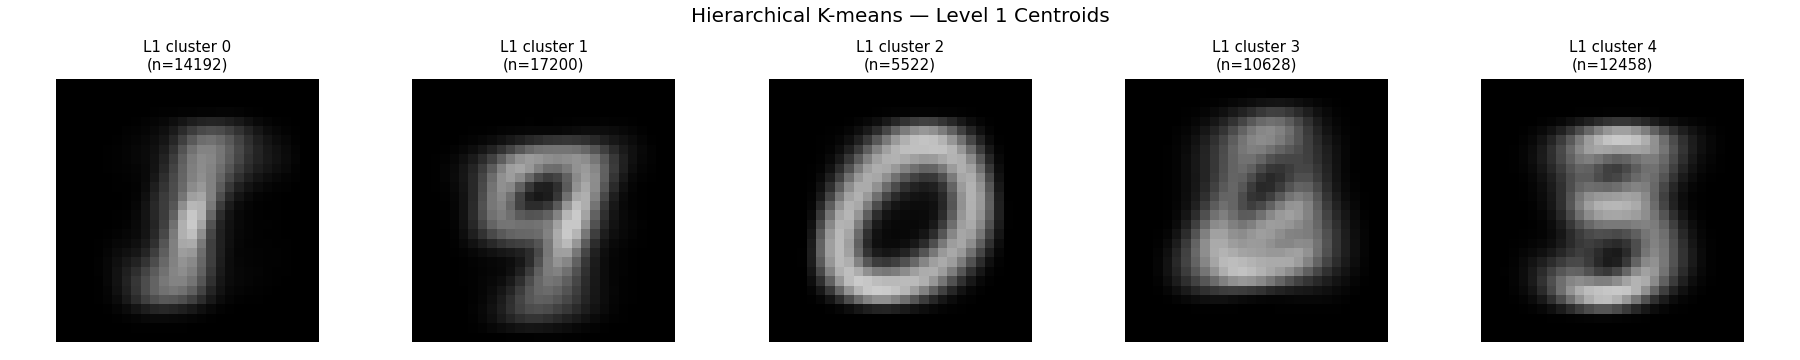
\includegraphics[width=0.9\textwidth]{plots/task4_level1_centroids.png}
    \caption{Level-1 centroids (coarse partition into 5 groups).}
    \label{fig:l1_centroids}
\end{figure}

\begin{figure}[H]
    \centering
    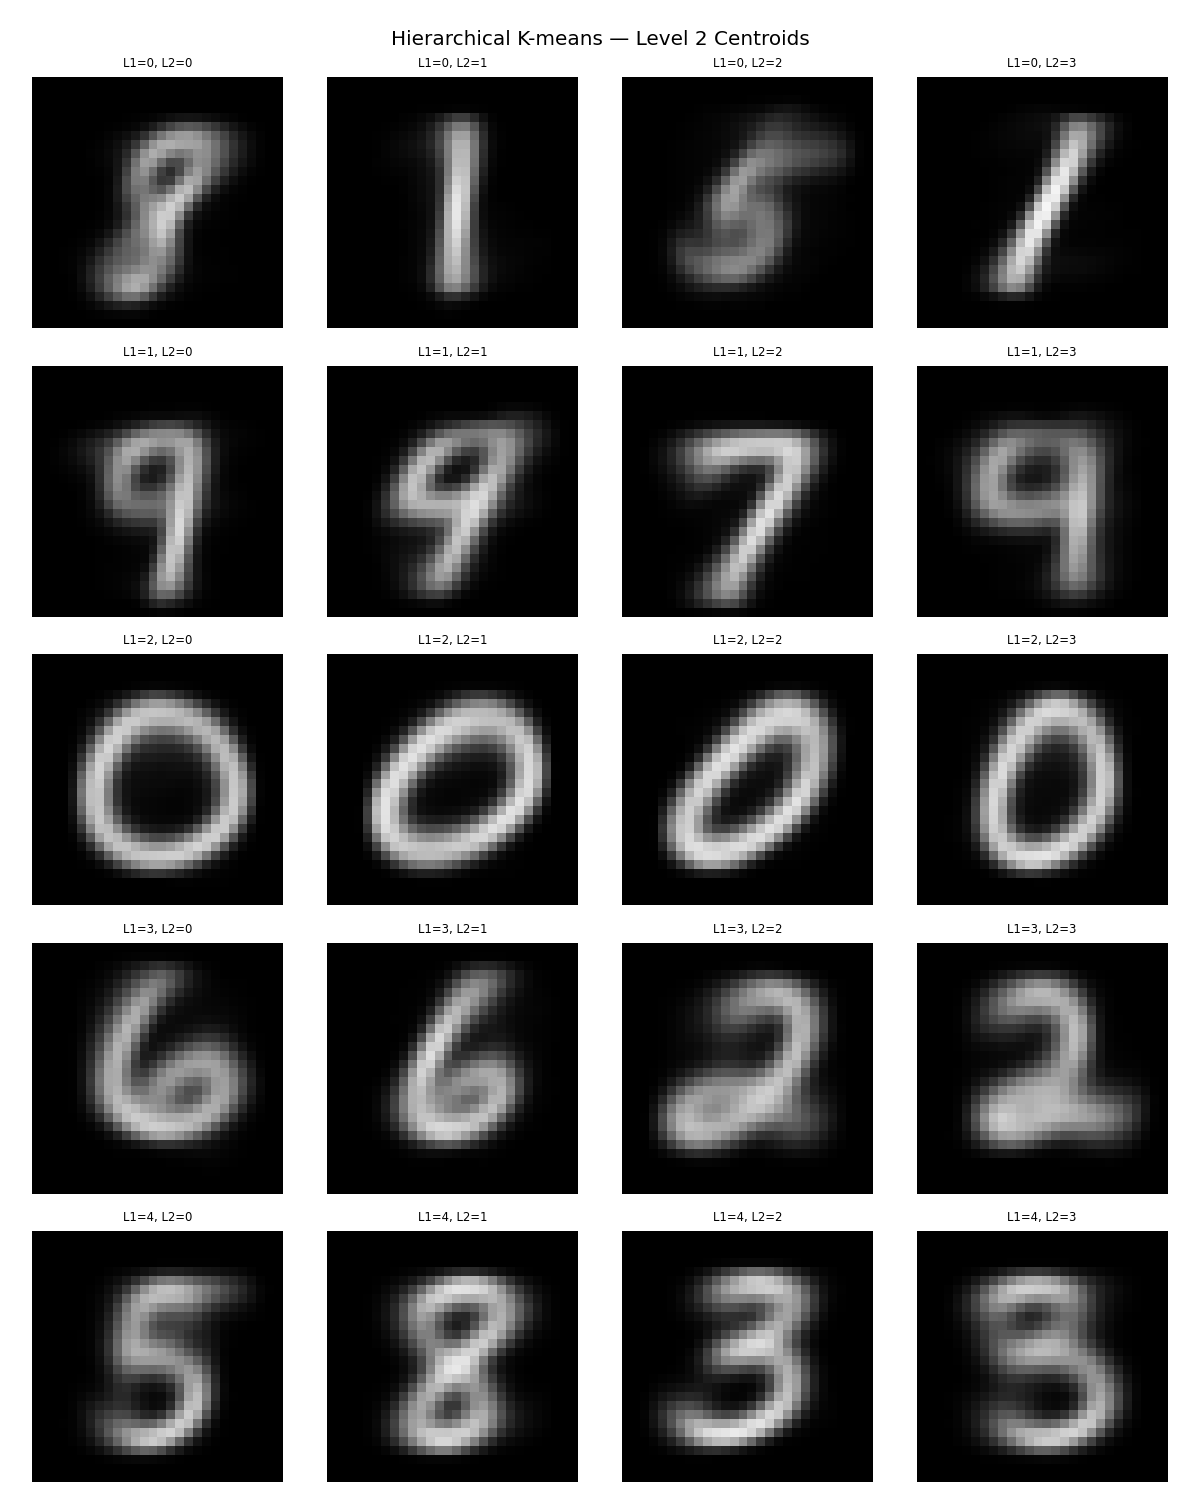
\includegraphics[width=\textwidth]{plots/task4_level2_centroids.png}
    \caption{Level-2 centroids: each row is a coarse cluster, each column a
    sub-cluster within it.}
    \label{fig:l2_centroids}
\end{figure}

\paragraph{Interpretability.}
Level-1 clusters correspond to broad visual categories (e.g., round shapes,
vertical strokes, complex multi-curve digits).
Level-2 clusters within each coarse group capture style variation: thick vs.\
thin strokes, slant direction, loop closure, etc.

\subsection{Digit Distribution in Level-1 Clusters}

\begin{figure}[H]
    \centering
    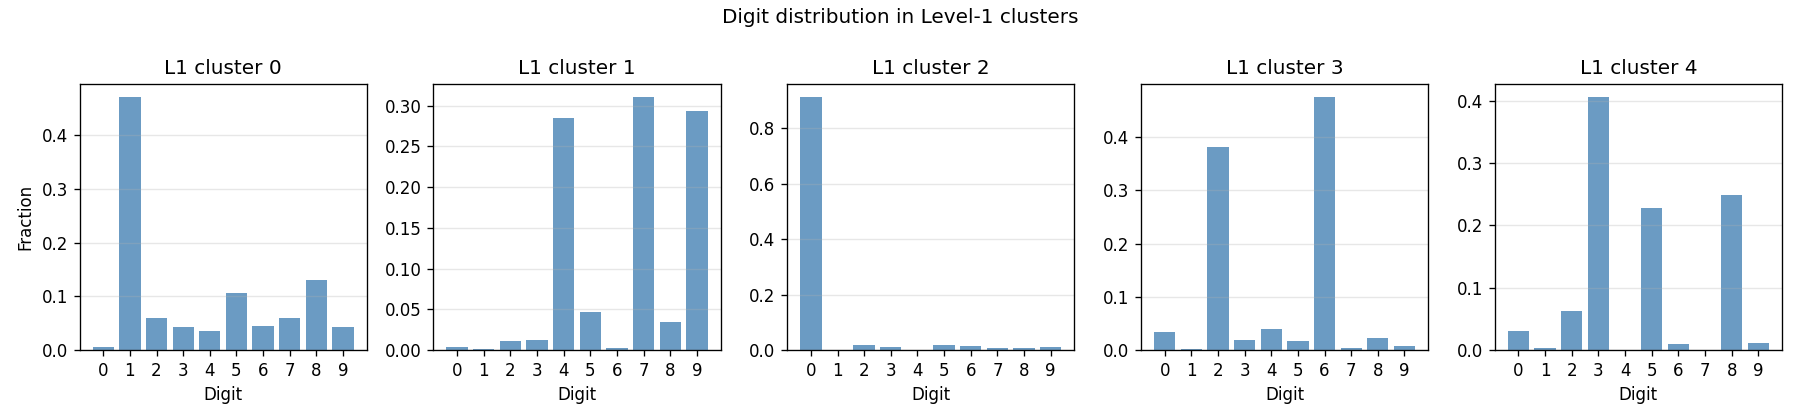
\includegraphics[width=\textwidth]{plots/task4_digit_distribution_l1.png}
    \caption{Digit distribution inside each level-1 cluster.}
    \label{fig:l1_digits}
\end{figure}

\subsection{Flat vs.\ Hierarchical Comparison}

\begin{figure}[H]
    \centering
    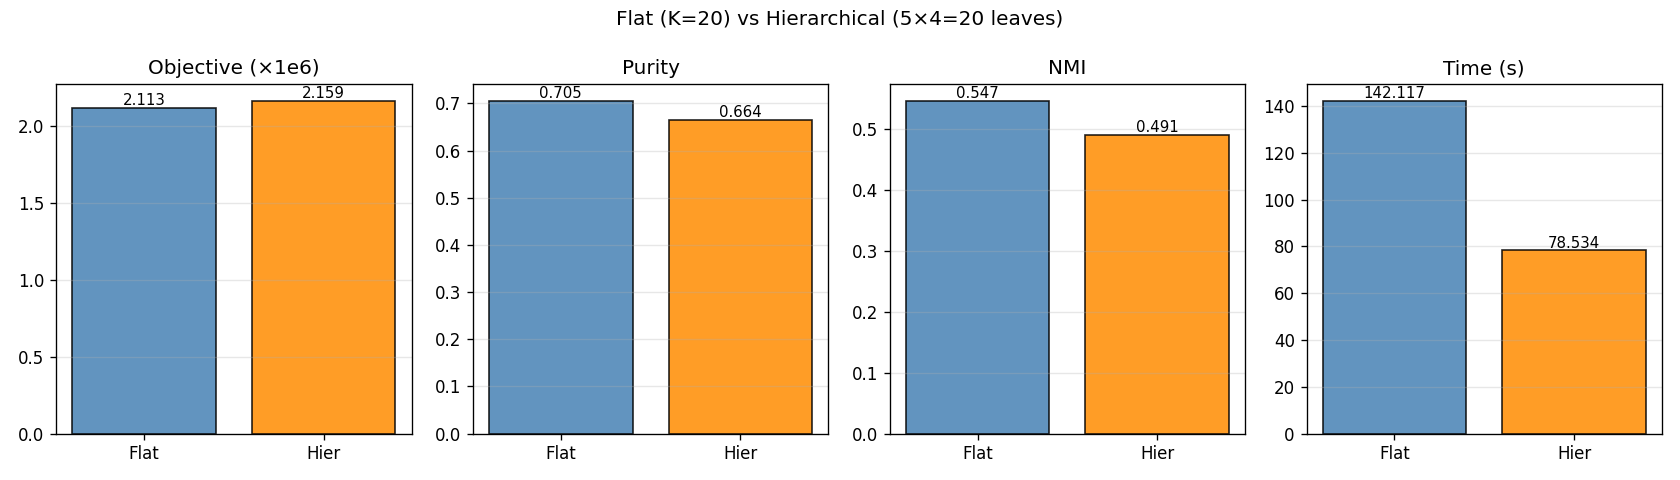
\includegraphics[width=\textwidth]{plots/task4_comparison.png}
    \caption{Flat K-means ($K{=}20$) vs.\ hierarchical K-means ($5\!\times\!4{=}20$ leaves).}
    \label{fig:task4_comparison}
\end{figure}

\paragraph{Quantitative comparison.}

\begin{table}[H]
    \centering
    \caption{Flat vs.\ hierarchical K-means at 20 leaf clusters.}
    \begin{tabular}{lrrrr}
        \toprule
        Method & Leaves & Objective & Purity & Time (s) \\
        \midrule
        Flat K-means ($K{=}20$)        & 20 & $2.113\times10^6$ & 0.705 & 142 \\
        Hierarchical ($5\!\times\!4$)  & 20 & $2.159\times10^6$ & 0.664 & \textbf{78} \\
        \midrule
        Flat K-means ($K{=}30$)        & 30 & $1.986\times10^6$ & 0.758 & $\sim$260 \\
        Hierarchical ($10\!\times\!3$) & 30 & $2.038\times10^6$ & 0.681 & $\sim$58 \\
        \bottomrule
    \end{tabular}
\end{table}

\paragraph{Discussion.}

\begin{itemize}[itemsep=3pt]
    \item \textbf{Speed.}
          Hierarchical K-means is $\approx$45\% faster at 20 leaves (78\,s vs 142\,s)
          and $\approx$4$\times$ faster at 30 leaves ($\sim$58\,s vs $\sim$260\,s).
          The reason: each level-2 sub-problem runs on 5\,000--17\,000 points
          with $K_2{=}3\text{--}4$, not 60\,000 points with $K{=}20\text{--}30$.
          The $\mathcal{O}(NKd)$ cost scales with the local cluster size.

    \item \textbf{Accuracy.}
          Flat K-means achieves lower objective ($\approx$2\% better) and higher
          purity ($\approx$6\% better) because it optimises the global criterion.
          Hierarchical K-means fixes level-1 centroids before level-2 runs;
          greedy errors at level 1 cannot be corrected.

    \item \textbf{Interpretability.}
          The tree structure provides a natural two-scale description.
          Level-1 clusters correspond to broad visual categories (round shapes,
          vertical strokes, etc.); level-2 clusters separate writing styles
          within each category.

    \item \textbf{Limitation.}
          Errors at level 1 propagate: a digit misassigned at the coarse
          level stays in the wrong branch through all subsequent splits.
          Without a global re-optimisation step, hierarchical greedy solutions
          cannot recover from early mistakes.
\end{itemize}

% ============================================================
\section{Task 5 — K-Medoids with Edit Distance}
% ============================================================

\subsection{Representation}

We converted each $28\!\times\!28$ image to a binary sequence using a pixel
threshold of 0.3, then applied run-length encoding (RLE) row by row.
The RLE sequence records alternating run lengths of background (0) and
ink (1) pixels; typical lengths are 20--60 for MNIST digits.

Figure~\ref{fig:task5_representations} shows the original image, the
binary threshold, the RLE histogram, and the flattened binary sequence for
three example images.

\begin{figure}[H]
    \centering
    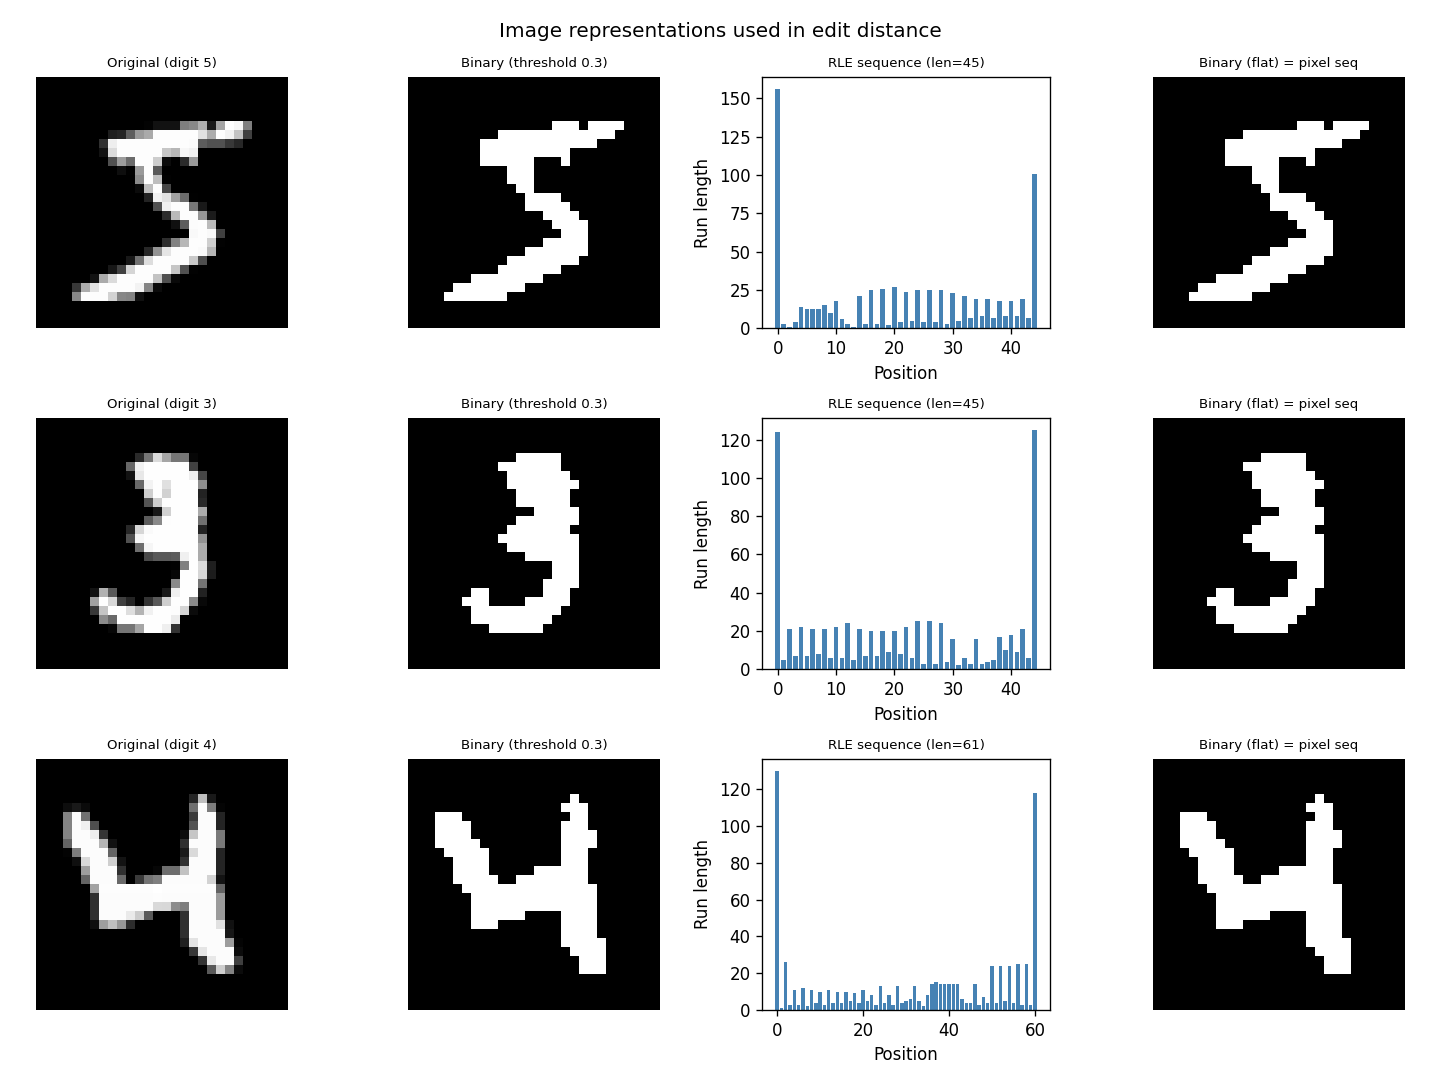
\includegraphics[width=\textwidth]{plots/task5_representations.png}
    \caption{Image representations for the edit-distance experiment.
    Columns: original, binary, RLE bar chart, binary sequence.}
    \label{fig:task5_representations}
\end{figure}

\subsection{Edit Distance}

We used the Levenshtein edit distance with unit insertion, deletion, and
substitution costs, computed via standard DP.
Pairwise distances for 500 images were pre-computed in $\mathcal{O}(N^2 L^2)$
time, where $L$ is the typical sequence length.

\subsection{Why the Standard K-Means Update Breaks}

The standard K-means centroid update is
\[
    \mu_k^{(t+1)} = \frac{1}{|C_k|} \sum_{i \in C_k} x_i.
\]
This is only meaningful when points are vectors in a Euclidean space: the
average is well-defined, is in the same space as the data, and minimises the
within-cluster SSE.

For sequences with edit distance, the ``average'' of two sequences is not
well-defined.
Even if it were, the result might not be a valid sequence.
The correct analogue is the \textbf{Fr\'echet mean}, which requires solving
a combinatorial problem (sequence alignment) over all cluster members.

We instead use \textbf{K-medoids}: the representative of each cluster is the
actual data point minimising the total edit distance to all other members.

\subsection{K-Medoids Algorithm}

\begin{enumerate}[itemsep=2pt]
    \item Initialise $K$ medoids by random selection.
    \item \textbf{Assignment:} assign each point to its nearest medoid under edit distance.
    \item \textbf{Update:} for each cluster, select the point minimising the
          total intra-cluster distance as the new medoid.
    \item Repeat until medoids stabilise.
\end{enumerate}

\subsection{Results}

\begin{figure}[H]
    \centering
    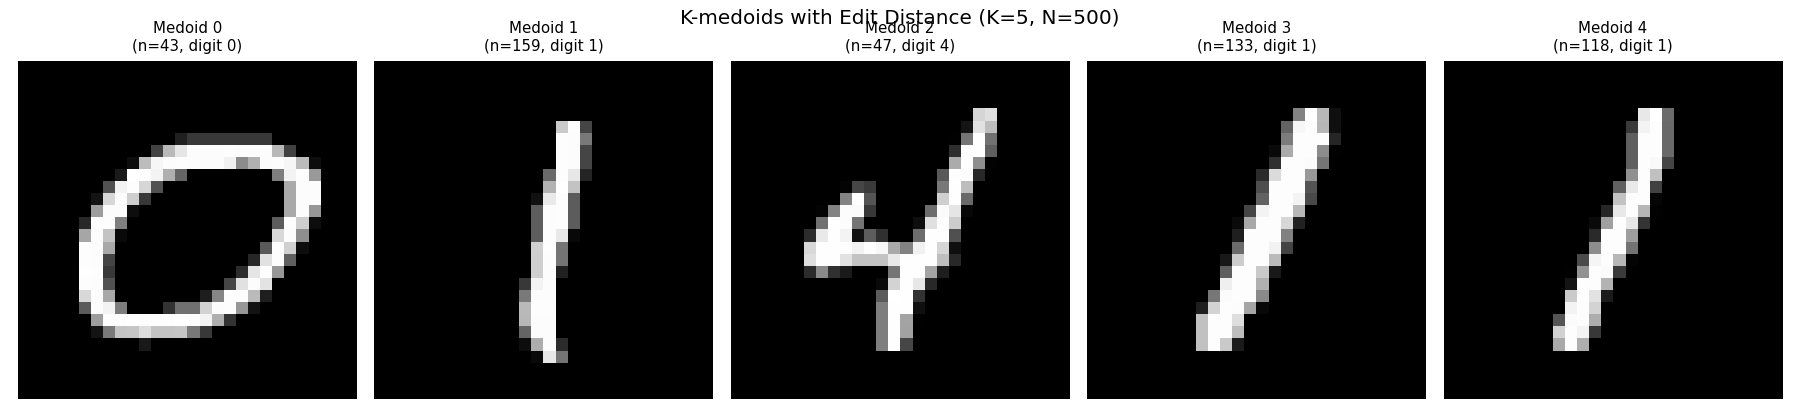
\includegraphics[width=0.9\textwidth]{plots/task5_medoids.png}
    \caption{K-medoids prototypes (actual training images) for $K{=}5$, $N{=}500$.}
    \label{fig:medoids}
\end{figure}

\begin{figure}[H]
    \centering
    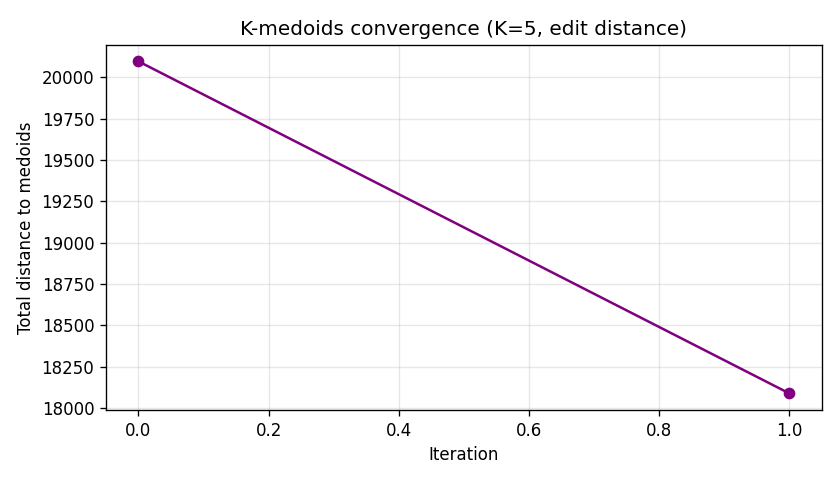
\includegraphics[width=0.65\textwidth]{plots/task5_kmedoids_convergence.png}
    \caption{K-medoids convergence: total distance to medoids per iteration.}
    \label{fig:kmedoids_conv}
\end{figure}

\begin{figure}[H]
    \centering
    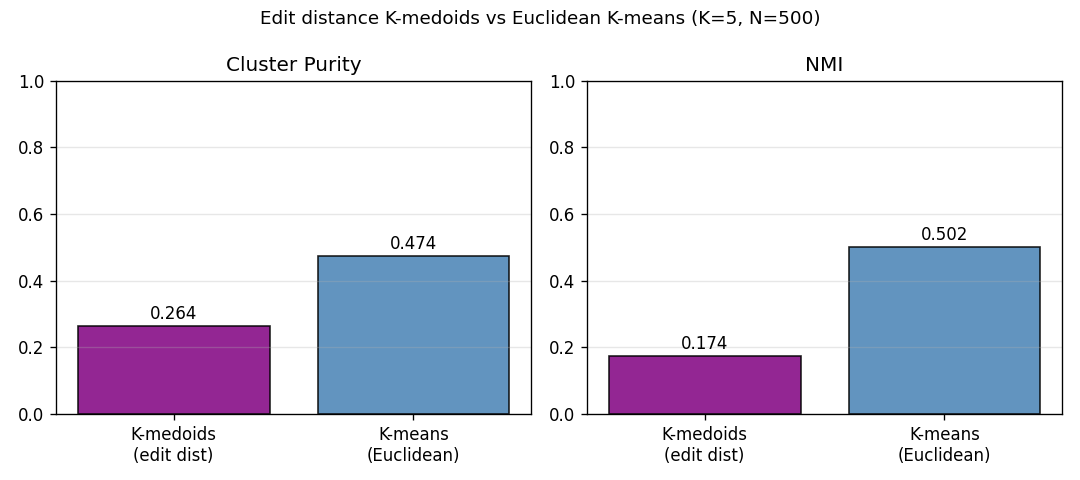
\includegraphics[width=0.7\textwidth]{plots/task5_comparison.png}
    \caption{Comparison of edit-distance K-medoids and Euclidean K-means on
    the same 500-image subset ($K{=}5$).}
    \label{fig:task5_comparison}
\end{figure}

\paragraph{Quantitative results.}

\begin{table}[H]
    \centering
    \caption{Edit-distance K-medoids vs.\ Euclidean K-means on 500 MNIST images ($K{=}5$).}
    \begin{tabular}{lrrr}
        \toprule
        Method & Purity & NMI & Distance pre-comp. \\
        \midrule
        K-medoids (edit distance) & 0.264 & 0.174 & 92.8\,s \\
        K-means (Euclidean)       & 0.474 & 0.502 & $<$1\,s \\
        \bottomrule
    \end{tabular}
\end{table}

\paragraph{Discussion.}

\begin{itemize}[itemsep=3pt]
    \item \textbf{Computational cost.}
          Pre-computing the $500 \times 500$ RLE edit distance matrix takes 93\,s.
          Scaling to 60\,000 images would require $\mathcal{O}(60000^2)$
          evaluations, taking roughly $93 \times (60000/500)^2 \approx 10^6$\,s
          ($\sim$10 days) --- totally prohibitive.

    \item \textbf{Quality.}
          Edit-distance K-medoids achieves substantially lower purity (0.264)
          and NMI (0.174) than Euclidean K-means (0.474/0.502) on the same 500
          images.
          The RLE edit distance is a poor proxy for visual digit similarity:
          a small vertical shift of the digit changes run lengths dramatically
          even though the digit class is the same.

    \item \textbf{Sensitivity to representation.}
          The RLE encoding collapses spatial structure into a 1D sequence.
          Two images of the same digit written at slightly different vertical
          positions can have very different RLE sequences, leading to large
          edit distances.
          More sophisticated representations (e.g., chain-code contours or
          structured patch descriptors) would improve the distance metric
          but at the cost of additional preprocessing.

    \item \textbf{Key insight.}
          Leaving the Euclidean setting removes two convenient properties:
          (1) the centroid update has a closed-form solution (the arithmetic mean),
          and (2) the objective decomposes cleanly across clusters.
          K-medoids preserves the cluster decomposition but increases the per-step
          cost from $\mathcal{O}(NK d)$ (K-means) to $\mathcal{O}(N^2)$ (medoid
          finding), making it impractical at scale without approximations
          such as PAM or CLARA.
\end{itemize}

% ============================================================
\section{Summary and Conclusions}
% ============================================================

\begin{table}[H]
    \centering
    \caption{Summary of clustering results across all tasks ($K{=}10$ or equivalent).}
    \label{tab:summary}
    \begin{tabular}{lccl}
        \toprule
        Method & Purity & NMI & Notes \\
        \midrule
        Pixel K-means ($K{=}10$)         & 0.590 & 0.489 & Baseline \\
        DFT K-means, flat weights        & 0.394 & 0.304 & Worse than pixel (phase lost) \\
        DFT K-means, low-pass ($\sigma{=}4$) & 0.431 & 0.359 & Best DFT variant (val set) \\
        Hierarchical K-means ($5\!\times\!4{=}20$) & 0.664 & 0.491 & 45\% faster, $-$6\% purity \\
        K-medoids edit dist ($K{=}5$, $N{=}500$) & 0.264 & 0.174 & RLE repr.; 93\,s for 500 pairs \\
        \bottomrule
    \end{tabular}
\end{table}

\paragraph{Key findings.}

\begin{enumerate}[itemsep=4pt]
    \item \textbf{Initialisation matters.}
          K-means\texttt{++} consistently produces lower final objectives than
          random initialisation, especially at large $K$.
          Practical rule: use 3--5 restarts with K-means\texttt{++}.

    \item \textbf{$K{=}10$ is natural but not always optimal.}
          The elbow and silhouette suggest $K{=}10$--$15$.
          Larger $K$ increases purity (finer-grained clusters) at the cost of
          interpretability; NMI plateaus around $K{=}20$.

    \item \textbf{DFT representation has mild benefits.}
          Log-magnitude DFT features are slightly more robust than raw pixels
          under train/test splits. Low-pass weighting is most useful when the
          task is to capture global digit shape rather than writer style.

    \item \textbf{Clusters generalise well.}
          Train and test metrics are nearly identical across all split ratios
          (50/50 to 90/10): pixel purity varies only $\pm$0.025 across ratios.
          Pixel clusters show higher variance across different random splits
          (std\,=\,0.035) but higher mean quality; DFT clusters are very stable
          (std\,=\,0.003) but consistently lower quality.

    \item \textbf{Hierarchical K-means trades optimality for speed and structure.}
          At 20 leaves: 45\% faster (78\,s vs 142\,s), $-$6\% purity (0.664 vs 0.705).
          The speed advantage grows with the number of leaves.
          The tree structure adds interpretability at the cost of greedy sub-optimality.

    \item \textbf{Edit distance breaks the K-means framework.}
          Without a well-defined notion of mean, the centroid update cannot be
          applied. K-medoids is the natural replacement, but its $\mathcal{O}(N^2)$
          distance-computation cost is prohibitive at scale (93\,s for 500 images;
          $\sim$10 days for 60\,000). Quality is also lower (purity\,=\,0.26 vs
          0.47 for Euclidean K-means) because the RLE edit distance is a poor
          proxy for visual digit similarity.
\end{enumerate}

\end{document}
